\documentclass[12pt] {article}
\usepackage{times}
\usepackage[margin=0.8in,bottom=1in,top=0.4in]{geometry}

\usepackage{hhline}
\usepackage{subfig}
\usepackage{amsmath}
\usepackage{amsfonts}
\usepackage[inline,shortlabels]{enumitem}%enumerate with letters
\usepackage{mathrsfs} 
\usepackage[square,numbers]{natbib}
\usepackage{graphicx}
\usepackage{natbib}


\begin{document}
\bibliographystyle{apalike}
\title{
Final Project -  EEC289Q \\
\begin{large}
Parallel Recursive Spoke Darts for Delaunay/Voronoi Meshing
\end{large}
}
\author{Ahmed H. Mahmoud, Muhammad Awad}
\date{}
\maketitle

%============Table========
%\begin{figure}[tbh]
% \centering    
%\begin{tabular}{ |p{4cm}|| p{2cm}|p{2cm}|p{2cm}|p{2cm}|}
% \hline
% & Processor 1 &  Processor 2  & Processor 3 & Processor 4\\ \hhline{|=|=|=|=|=|}
% \hline
% Performance          &$1.08$        &$1.425$       &\textbf{1.52}  &   \\
% \hline
%\end{tabular} 
%\caption{Metric table for the four processors}
%   \label{tab:metric}
%\end{figure} 
%============Figure========
%\begin{figure}[!tbh]
%\centering        
%   \subfloat {\includegraphics[width=0.65\textwidth]{fig2_4.png}}
%   \caption{ }
%   \label{fig:fig}
%\end{figure}

%\begin{enumerate}[(a)]
%\end{enumerate}

\section*{Abstract}
We propose to implement the Recursive Spoke Darts (RSD) algorithm; a local hyper-plane sampling method for 3D Delaunay and Voronoi meshing presented in \citep{EBEIDA2016110}. The algorithm has two objectives. Through reliance on simple local operations (recursive line-plane trimming) and with zero-communication between vertices, the algorithm presents the first truly scalable Delaunay triangulation. However, the algorithm was only implemented on MPI settings where it improves over the state-of-the-art. The improvement comes in terms of speedup and the ability to construct the mesh exactly in higher dimensions where other methods give approximate solution, prohibitively slow or fail completely. In this project, we implemented RSD algorithm in 3D space by mapping it into the GPU. 

%\section*{Introduction:}
%Delaunay Triangulation (DT) of a point set has important applications in many fields including data visualization and imaging, terrain modeling, finite element mesh generation, surface reconstruction, and structural networking for arbitrary point sets. This is due to its nice geometric properties and desirable qualities. For example, in $\mathbb{R}^{3}$, DT minimizes the maximum radius of the minimum containment sphere of the tetrahedra which guarantees the convergence of the finite element solution. Accelerating the computation of DT is a necessity with the rapid increase in the problem size from thousands of points to millions and even billions~\citep{lo20153d}. 

%There has been a decent amount of work devoted to parallelize the DT computation most of which is an adaption of one of the serial algorithms. Examples include parallelize Dwyer's divide and conquer algorithm~\citep{fuetterling2014high, cignoni1998dewall, 574023, lo20153d}, incremental/point insertion algorithm~\citep{cao2014gpu, batista2010parallel} and flipping algorithms~\citep{liparulo2015fuzzy}. Even though all these implementations have achieved good speedup over the serial counterparts, we hypothesize that in order to further accelerate the computation, one should start with an algorithm that is designed for parallel execution. RSD has the potential to be the first DT algorithm that is deigned with parallel mindset. RSD abandons the dependence on the empty sphere principle which gives it the foundation needed for scalable consistent meshing. Additionally, the simple operations the RSD algorithm relies on make it more favorable for GPU settings. 

\section*{Algorithm Overview}
\paragraph{Definitions:}
\begin{itemize}
\item \textit{Spoke:} a ray that later gets trimmed to a line-segment.
\item \textit{Voronoi plane:} a 3D plane defined by points $p$ and $q$ such that the plane passes by the mid-point between $p$ and $q$ and the line between them is normal to the plane.
\end{itemize}

The input to the algorithm is a set of samples in 3D space. The algorithm processes all samples independently in parallel. For each sample, the algorithm has two phases; \emph{explore} and \emph{propagate}. For each sample $x_{0}$, we do
 
\begin{itemize}
\item \textbf{Explore:}
\begin{enumerate}
\item Sample a random 3-d spoke $s_{0}$ in 3D space starting from $x_{0}$. Trim $s_{0}$ by Voronoi planes of $x_{0}$'s neighbor samples with $x_{0}$. Record the neighbor $n_{0}$ that trims $s_{0}$ the shortest and its Voronoi cutting plane $p_{0}$. 
\item Sample random 2-d spoke $s_{1}$ on the cutting plane $p_{0}$ starting from the end point of $s_{0}$. Trim $s_{1}$ by Voronoi planes of $x_{0}$'s neighbor samples with $x_{0}$ ignoring $n_{0}$. Record the neighbor $n_{1}$ that trims $s_{1}$ the shortest and its Voronoi cutting plane $p_{1}$. 

\item  Sample random 1-d spoke $s_{2}$ starting from the end point of $s_{1}$ along the intersection of $p_{0}$ and $p_{1}$. Trim $s_{2}$ by Voronoi planes of $x_{0}$'s neighbor samples with $x_{0}$ ignoring $n_{0}$ and $n_{1}$. Record the neighbor $n_{2}$ that trims $s_{2}$ the shortest and its Voronoi cutting plane $p_{2}$. The end point of $s_{2}$ is a true Voronoi vertex $v_{0}$ and the tuple $\left\langle x_{0}, n_{0}, n_{1}, n_{2} \right\rangle$ is a Delaunay tetrahedron. 
\end{enumerate}
\end{itemize}

\begin{itemize}
\item \textbf{Propagate:}
\begin{enumerate}
\item Sample three deterministic 1-d spokes starting from $v_{0}$ along the line of intersection of $p_{0}$-$p_{1}$, $p_{1}$-$p_{2}$, and $p_{0}-p_{2}$. Figure~\ref{fig:algo} shows the direction of the spokes. Trim the three spokes by Voronoi planes of $x_{0}$'s neighbor samples with $x_{0}$ ignoring any the two neighbor samples that identify the Voronoi planes along which the spoke is sampled. The end point of each trimmed spoke is a true Voronoi vertex. 
\item Keep sampling deterministic 1-d spokes from the discovered Voronoi vertices in the same fashion as 1. Terminate when search path when two spokes meet at the same Voronoi vertex.  
\end{enumerate}
\end{itemize}

\begin{figure}[!tbh]
\centering        
   \subfloat {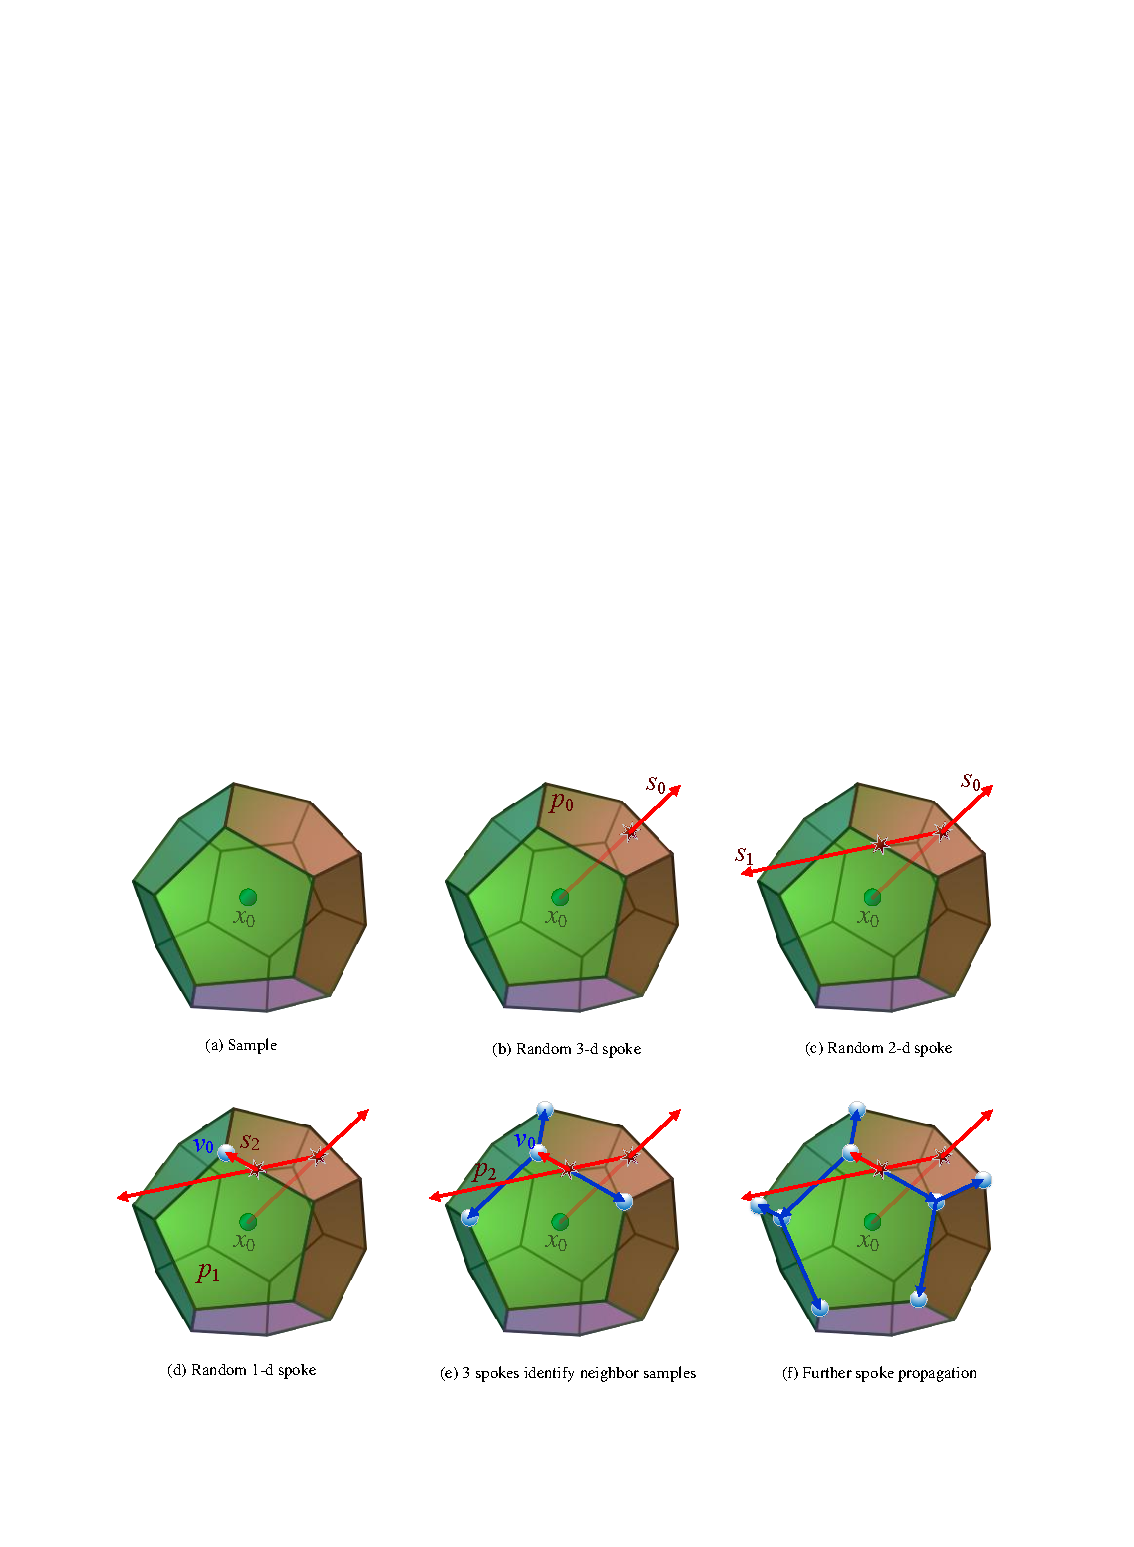
\includegraphics[width=\textwidth]{algo.pdf}}
   \caption{Overview of the RSD algorithm in 3D. From a-d is the \emph{Explore} phase, e-f is the \emph{Propagate} phase.}
   \label{fig:algo}
\end{figure}

\section*{Algorithm Details}
Here we describe the details and how we map the algorithm into the GPU. 
We can achieve the coalescing behavior if neighbor samples in the spatial domain are also neighbor in the memory layout i.e., the difference between indicies is small. This is because every sample need to read the coordinates of its neighbour samples. We achieve this by building a balanced kd-tree on the CPU side during which we re-order the sample indices. Figure~\ref{fig:tree} shows the effect of reordering. The kd-tree is also used to range-query the neighbor of each sample. Thus, the input of the kernel is the input sample index and a list of its neighbor samples. 

For the sake of simplicity, we assume the point is in general position which can be achieved by random sampling. From that we can assume the maximum number of Delaunay edges of a sample is bounded. We set this bound to 32 for pre-allocation of memory for the output. 

\begin{figure}[!tbh]
\centering        
   \subfloat [Input] {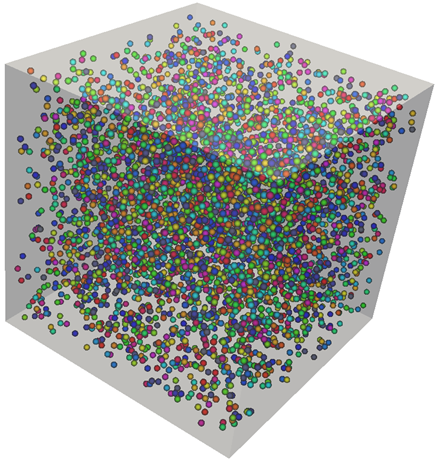
\includegraphics[width=0.35\textwidth]{tree_before.png}}
   \subfloat [Reordered] {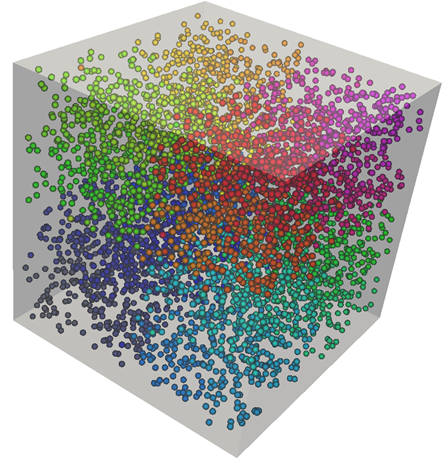
\includegraphics[width=0.35\textwidth]{tree_after.png}}
   
     \subfloat [Input] {
\includegraphics[width=0.35\textwidth]{matrix_unbalanced.png}}
   \subfloat [Reordered] {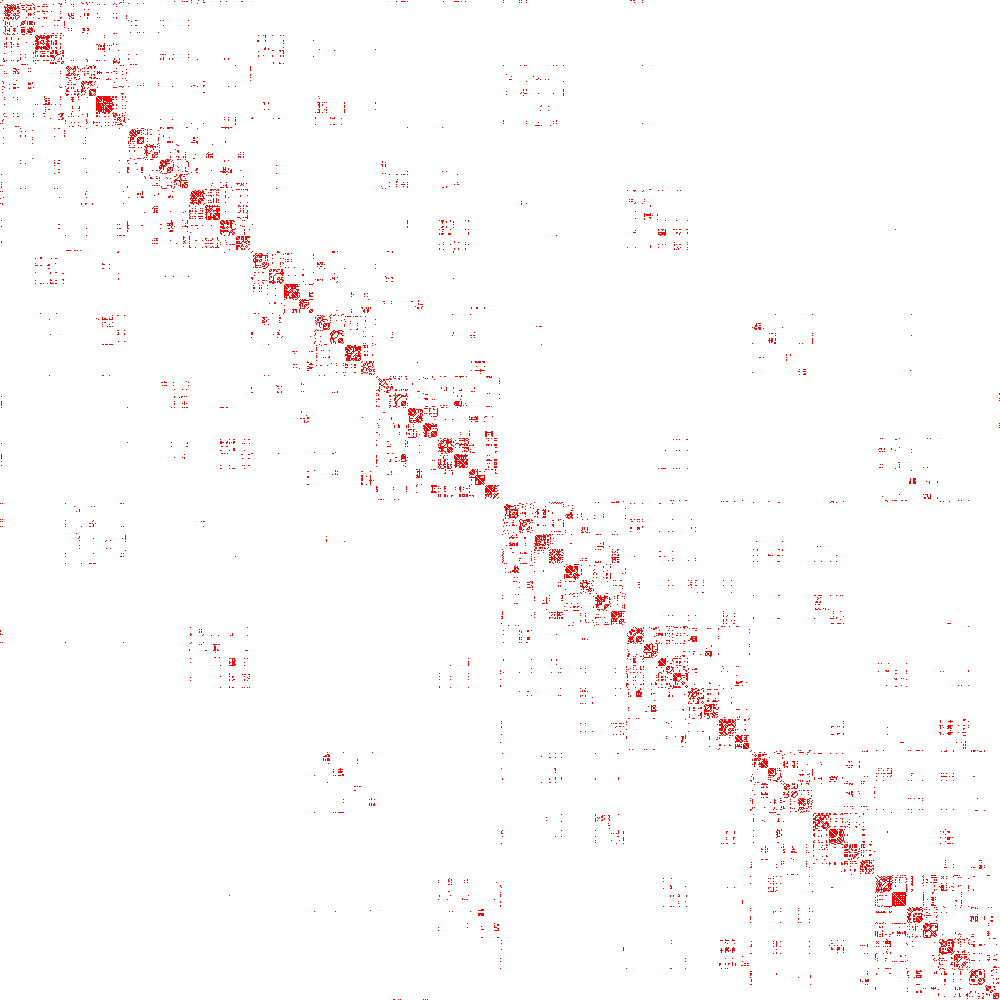
\includegraphics[width=0.35\textwidth]{matrix_balanced.png}}
  
   \caption{Top: The effect of reordering the samples while building the balanced Kd-tree (samples indices are encoded using color). Bottom: Adjacency matrix after reordering showing better locality compared to the initial input.}
   \label{fig:tree}
\end{figure}


We choose to process each sample using one thread. Since the distribution of the samples is nearly uniform, the load imbalance is eliminated. However, the thread divergence was harder to eliminate due to the following 
\begin{enumerate}
\item Number of neighbors returned from the range query varies from one sample to another. 
\item The number of edges and faces for each sample in the output varies. This can cause more than two-way thread divergence within a warp. 
\end{enumerate}

We can eliminate the first by making sure all samples will have the same number of neighbors by padding. We noticed that the thread divergence cause by the second was more severe. 

We choose to use small blocks such i.e., 32-64 threads per block. This helped us load all the information to shared memory in coalesced manner as much as possible. Larger blocks also sometimes were not feasible since the kernel requires many registers to do all the geometric work. 

\section*{Results}

We compare our implementation performance with gStar4D~\citep{Ashwin2012GPUDelaunay}, a CUDA implementation of the gStar4D algorithm. The testing platform uses a Tesla K40c GPU. Figure~\ref{fig:timing} shows that our implementation achieves $\approx4$x speed up over gStar4D. *Why? what do they do?*

\begin{figure}[!tbh]
\centering        
   \subfloat {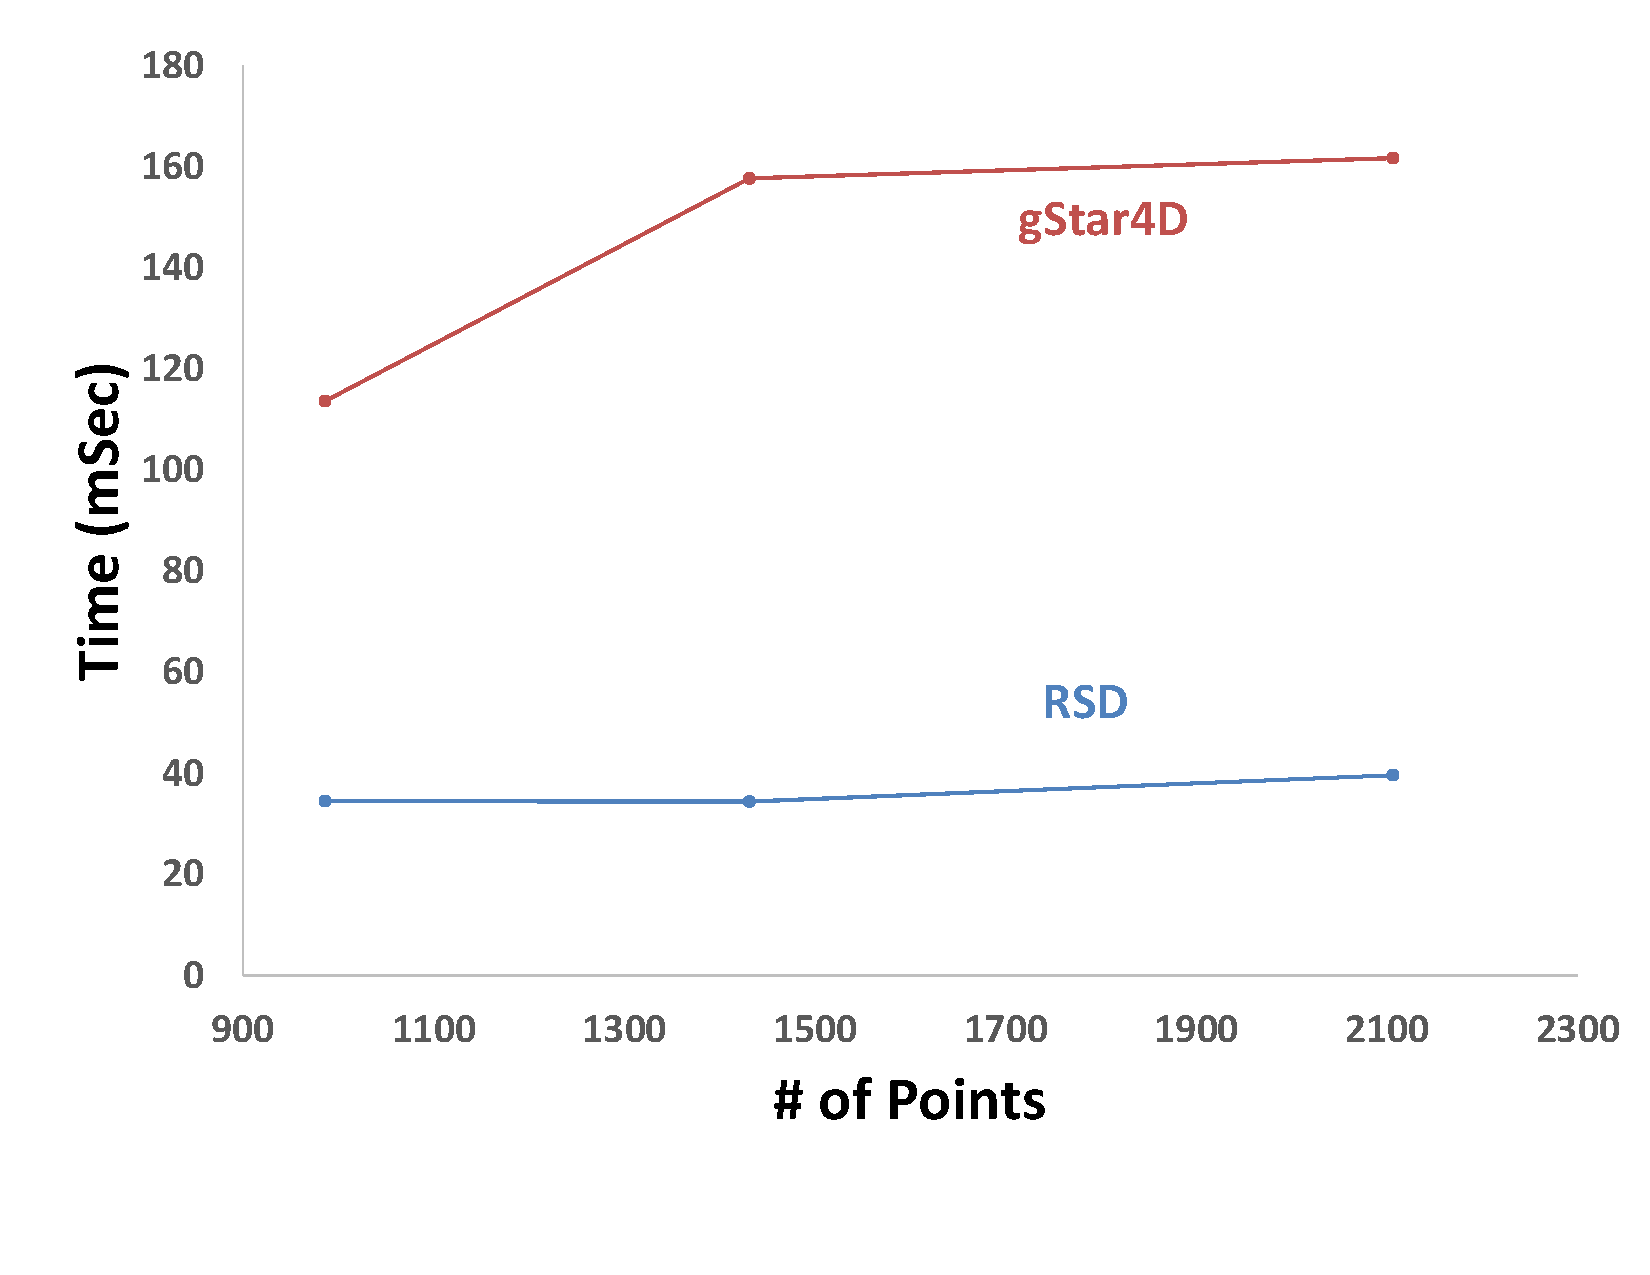
\includegraphics[width=0.8\textwidth]{timing.pdf}}
   \caption{Our performance compared to gStar4D.}
   \label{fig:timing}
\end{figure}

\bibliography{mybib}
\end{document}